\documentclass[11pt,a4paper]{article}

% --- Packages ---
\usepackage[utf8]{inputenc}
\usepackage[T1]{fontenc}
\usepackage{geometry}
\geometry{margin=2cm}
\usepackage{array}
\usepackage{fancyhdr}
\usepackage{titlesec}
\usepackage{tcolorbox}
\tcbuselibrary{listings,skins,breakable}
\usepackage{amsmath,amssymb}
\usepackage{float}
\usepackage{xurl}
\usepackage[hidelinks]{hyperref}
\usepackage{graphicx}
\usepackage{subcaption}
\usepackage[english]{babel}
\usepackage{mwe}

\lstdefinestyle{pythonstyle}{
  language=Python,
  backgroundcolor=\color{gray!5},
  basicstyle=\ttfamily\small,
  keywordstyle=\color{blue}\bfseries,
  commentstyle=\color{gray}\itshape,
  stringstyle=\color{teal},
  numberstyle=\tiny\color{gray},
  numbers=left,
  stepnumber=1,
  numbersep=8pt,
  showspaces=false,
  showstringspaces=false,
  showtabs=false,
  tabsize=4,
  breaklines=true,
  breakatwhitespace=true,
  frame=single,
  rulecolor=\color{gray!40},
  captionpos=b,
  keepspaces=true,
  morekeywords={ceil,cbrt,round,split,Node},
}

\hypersetup{
    pdftitle={A New Curriculum},
    pdfauthor={Ludwig Alvarado},
    pdfsubject={Ejercicio de invertir una lista enlazada},
    pdfkeywords={estructuras de datos,prueba,programación},
    pdfcreator={GNU Emacs desde Arch (btw) GNU/Linux y LaTeX con hyperref},
    pdfproducer={pdflatex}
}


% --- Formatting ---
\pagestyle{fancy}
\fancyhf{}
\setlength{\headheight}{30pt}
\setlength{\footskip}{20pt}
\setlength{\parindent}{0pt}
\setlength{\parskip}{0.7em}

% Left header (university and exam info)
\rhead{%
   \small
   Universidad Jorge Tadeo Lozano\\
   Data Structures - Group 2\\
   Programming Test 
}

% Right header (date, professor, monitor)
\lhead{%
   \small
   \textbf{Fecha}: \today \\
   \textbf{Professor:} José Alejandro Franco Calderón \\
   \textbf{Assistant:} Ludwig Alvarado Becerra
}

\cfoot{\thepage}

\titleformat{\section}{\large\bfseries}{\thesection.}{0.5em}{}

% --- Environment for samples ---
\newenvironment{sample}[2]{
  \begin{tcolorbox}[title=Test \##1, colback=white, colframe=black, sharp corners,
    fonttitle=\bfseries, breakable]
    \begin{tabular}{|p{0.45\linewidth}|p{0.45\linewidth}|}
      \hline
      \textbf{Input} & \textbf{Output} \\
      \hline
      }{\\ \hline
    \end{tabular}
  \end{tcolorbox}
}

% --- Document ---
\begin{document}

\begin{center}
  {\LARGE \bf A New Curriculum}\\[1ex]
  Author: Ludwig Alvarado Becerra
\end{center}

Universities often need to update their academic curricula. At the University of Typing and Drinking Energy Drinks Overnight (UTADEO), the Systems Engineering curriculum is represented as a singly linked list of courses.


\begin{figure}[h]
    \centering
    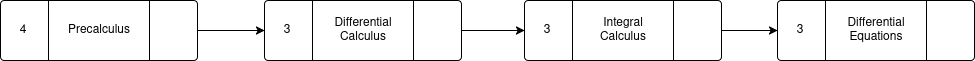
\includegraphics[width=\textwidth]{img/pic1.png}
    \caption{Calculus and mathematics line in UTADEO}
    \label{fig:calculus}
\end{figure}

Each course contains three fields:

\begin{itemize}
  \item \texttt{Name}: the course title
  \item \texttt{Credits}: number of academic credits
  \item \texttt{Link}: pointer to the next course in the sequence
\end{itemize}


The \texttt{Link} field also indicates a prerequisite relationship: if course \texttt{A} links to course \texttt{B}, then \texttt{A} must be completed before taking \texttt{B}.

For example, in figure~\ref{fig:calculus}:

\begin{itemize}
  \item \texttt{Name} = Precalculus
  \item \texttt{Credits} = 4
  \item \texttt{Link} -> Differential Calculus
\end{itemize}

This means that Precalculus is a prerequisite for Differential Calculus.

Unfortunately, during the last curriculum update, some administrators accidentally stored the course list in reverse order. As a result, students may be asked to take advanced courses before introductory ones.

Your task is to restore the correct prerequisite order by reversing the incorrectly ordered linked list.

\subsection*{Input}

The judge provides a curriculum already loaded in memory as a singly linked list.  
You are given access to its first node, which is an instance of class \texttt{Node}.  
Each node stores three private attributes:

\begin{itemize}
    \item \texttt{Name}: course title
    \item \texttt{Credits}: number of academic credits
    \item \texttt{Link}: reference to the next course in the sequence
\end{itemize}

Direct access to these attributes is forbidden. All interaction with the structure must be performed through the provided getters and setters:

\begin{itemize}
  \item \lstinline[style=pythonstyle]|set_name(new_name: str)|  
  Updates the current course title.

  \item \lstinline[style=pythonstyle]|get_name()|  
  Returns the current course title.

  \item \lstinline[style=pythonstyle]|set_credits(new_credits: int)|  
  Updates the credits of the current course.

  \item \lstinline[style=pythonstyle]|get_credits()|  
  Returns the credits of the current course.

  \item \lstinline[style=pythonstyle]|set_next(next_course: Node)|  
  Redirects the current link to another node.

  \item \lstinline[style=pythonstyle]|get_next()|  
  Returns the next node in the sequence, or \texttt{None} if the node is the tail.
\end{itemize}

The list contains exactly \(N\) nodes, where:

\[
2 \leq N \leq 10^7
\]

The courses currently appear in the wrong order.  
The first provided node corresponds to the course that should appear last in the corrected curriculum.

No additional guarantees are given about course names or credits beyond being valid values.

\subsection*{Output}

Reconstruct the curriculum so that prerequisite relations are restored and the sequence becomes academically consistent.

After modifying the structure, the final curriculum must be shown using the public method:

\lstinline[style=pythonstyle]|print_list()|

This method prints the nodes from the current head following their \texttt{Link} references until the end of the list.

Your solution is expected to transform the existing linked structure itself rather than rebuilding an unrelated one.

Any output not generated through the final valid structure may be ignored by the judge.

\subsection*{Note}

You don't have to worry about the implementation of all the functions mentioned, assume they are already working properly.

\subsection*{Sample Cases}



\begin{sample}{1}{}
  \texttt{Differential Equations}

  &
  \texttt{Precalculus -> Differential Calculus -> Integral Calculus -> Differential Equations}

\end{sample}
 

\subsection*{Important Aspects}

The following points describe how this exam problem will be evaluated and what restrictions must be considered during the solution process:

\begin{enumerate}

\item The test will be solved in \textbf{two stages}:

\begin{itemize}
    \item Design and explanation of the algorithm on paper \textbf{(3.0 points)}.
    \item Correct implementation in the code editor \textbf{(2.0 points)}.
\end{itemize}

Both stages are graded independently. A correct idea with poor implementation, or correct code with no reasoning, may lose points.

\item This exercise evaluates topics studied up to \textbf{singly linked lists}, including:

\begin{itemize}
  \item Traversal
  \item Pointer/reference manipulation
  \item Node relinking
  \item Iterative control structures
  \item Stacks and queues.
\end{itemize}

\item Since the list may contain up to \(10^7\) nodes, your solution must be efficient.

Algorithms with repeated traversals, unnecessary copying, or quadratic behavior may fail practical evaluation. 

\item The intended solution modifies the existing structure by changing links between nodes.

\item You are expected to use only the methods already provided in the statement:

\begin{itemize}
    \item \lstinline[style=pythonstyle]|get_next()|
    \item \lstinline[style=pythonstyle]|set_next(...)|
    \item and the remaining getters/setters when needed
\end{itemize}

Direct access to private attributes is considered incorrect.

\item No external libraries are required for this problem.

If your solution depends on advanced modules or imported data structures, it is likely not the intended approach.

\item You may assume that the initial linked list is valid:

\begin{itemize}
    \item It contains exactly \(N\) nodes.
    \item The final node points to \texttt{None}.
    \item There are no broken references.
\end{itemize}

Therefore, no defensive validation is necessary.

\item The final output must be generated only through:

\lstinline[style=pythonstyle]|print_list()|

Manual printing of names or custom formatting does not replace the required final structure.

\item Output format must match exactly the judge expectation.

Any missing links, extra spaces, duplicated nodes, infinite loops, or incorrect termination will be judged as wrong answer.

\end{enumerate}





\end{document}
